\documentclass[12pt,letterpaper]{article}

\usepackage[brazilian]{babel}
\usepackage[utf8]{inputenc}
\usepackage[T1]{fontenc}

\usepackage{fullpage}
\usepackage{cancel}
\usepackage[top=2cm, bottom=4.5cm, left=2.5cm, right=2.5cm]{geometry}
\usepackage{amsmath,amsthm,amsfonts,amssymb,amscd}
\usepackage{lastpage}
\usepackage{enumerate}
\usepackage{fancyhdr}
\usepackage{mathrsfs}
\usepackage{xcolor}
\usepackage{graphicx}
\usepackage{listings}
\usepackage{hyperref}

\hypersetup{%
	colorlinks=true,
	linkcolor=blue,
	linkbordercolor={0 0 1}
}

\setlength{\parindent}{0.0in}
\setlength{\parskip}{0.05in}

% Edit these as appropriate
\newcommand\course{Rener Oliveira}
\newcommand\lcur{\mathcal{L}}
\newcommand{\real}{\mathbb{R}}
\newcommand{\rr}{\mathbb{R}^2}
\newcommand{\rn}{\mathbb{R}^n}
\newcommand{\linesep}{{\color{black} \rule{\linewidth}{0.5mm} }}
\newcommand{\rpos}{\mathbb{R}_{>0}}
\newcommand{\ex}[1]{\textcolor{blue}{\textbf{Exercício #1}}}
\newcommand{\sol}[1]{\textbf{Solução #1}}
\newcommand{\blue}[1]{{\color{blue}{#1}}}
\newcommand{\bd}[1]{\boldsymbol{#1}}
\pagestyle{fancyplain}
\headheight 35pt        
\chead{\textbf{\Large Lista 3 \\ Curvas e Superfícies}}
\rhead{\small{\course \\ \today}}
\lfoot{}
\cfoot{}
\rfoot{\small\thepage}
\headsep 1.5em

\begin{document}
	
	\begin{enumerate}
		
		\item [\ex{1}] \textcolor{blue}{Verifique a regularidade e calcule o comprimento de arco e a curvatura das seguintes curvas, quando possível:}
		
		
		\begin{itemize}
			\blue{
			\item (retas) $\alpha(t)=(a+ct,b+dt),t\in\mathbb{R};$}
		
			Verificando regularidade:
			
			$\alpha'(t)=(c,d)$, que é diferente do vetor nulo para todo $t$, desde que $c$ e $d$ não sejam ambos nulos, pois neste caso não se trataria de um reta, mas sim de um ponto isolado. \textbf{Logo $\alpha$ é regular.}
		
			
			Calculando o comprimento de arco:
			
			\begin{align*}
				\displaystyle\lcur(t)&=\int_{t_0}^t||\alpha'(u)||du\\
				&=\int_{t_0}^t||(c,d)||du\\
				&=\int_{t_0}^t\sqrt{c^2+d^2}du\\
				&(t-t_0)\sqrt{c^2+d^2}
			\end{align*}
		
		Para a curvatura, vamos reparametrizar $\alpha$ por $\lcur(t)$ e calcular $\kappa(s)=\det(\alpha'(s),\alpha''(s))$ após a reparametrização.
		
		Para facilitar as contas, façamos $t_0=0$.
		
		\begin{align*}
			\alpha(\lcur^{-1}(t))&=(a+ct/\sqrt{c^2+d^2},b+dt/\sqrt{c^2+d^2})\\
			\alpha'(s)&=(c/\sqrt{c^2+d^2},d/\sqrt{c^2+d^2})\\
			\alpha''(s)&=(0,0)\Rightarrow\\
			\kappa(s)&=\det(\alpha',\alpha'')=0
		\end{align*}
		
		\blue{
			\item $\alpha(t)=(t,t^4),t\in\mathbb{R};$}
		
		Verificando regularidade:
		
		$\alpha'(t)=(1,4t^3)\neq0$, pois a primeira componente é constante não-nula. \textbf{Logo a curva é regular.}
		
		Calculando o comprimeiro de arco:
		\begin{align*}
			\displaystyle\lcur(t)&=\int_{t_0}^t||\alpha'(u)||du\\
			&=\int_{t_0}^t||(1,4u^3)||du\\
			&=\int_{t_0}^{t}\sqrt{16u^6+1}du
		\end{align*}
	
		Para a curvatura vamos usar a Proposição 2.2.1 de \cite{pressley2001elementary}, que nos dá uma fórmula para curvatura de uma curva regular qualquer\footnote{Na verdade a referência usa norma no produto vetorial no numerador, que no caso é equivalente ao determinante.}.
		
		
		No nosso caso, a curvatura será:
		 
		 \begin{align*}
		 	\kappa(s)&=\dfrac{\det(\alpha'(s),\alpha''(s))}{||\alpha'(s)||^3}\\
		 	&=\dfrac{\det[(1,4s^3);(0,12s^2)]}{(1+16s^6)^{3/2}}\\
		 	&=\dfrac{12s^2}{(1+16s^6)^{3/2}}
		 \end{align*}
	 		
	 
		\blue{
			\item (círculos) $\alpha(s)=(a+r\cdot\cos(s/r),b+r\cdot\sin(s/r)), s\in\mathbb{R},r>0;$}
		
		Verificando regularidade:
		
		$\alpha'(s)=(-r\cdot\sin(s/r)\cdot1/r,r\cdot\cos(s/r)\cdot1/r)\\=(-\sin(s/r),\cos(s/r))$
		
		Tal velocidade será sempre diferente do vetor nulo, pois os pontos na qual a primeira coorderada zera pertence ao conjunto $A=\{rk\pi;k\in\mathbb{Z}\}$, ou seja, os múltiplos de $0$ e $\pi$ radianos do círculo trigonométrico (ajustado por r);
		
		Já os pontos que a segunda componente zera pertencem à $B=\{r\pi/2+rk\pi;k\in\mathbb{Z}\}$.
		
		Se $s\in A$, $\alpha(s)=(0,1)$ para $k$ par e $\alpha(s)=(0,-1)$ para $k$ ímpar.
		
		Se $s\in B$, $\alpha(s)=(1,0)$ para $k$ par e $\alpha(s)=(-1,0)$ para $k$ ímpar.
		
		\textbf{Logo o círculo é regular}
		
		Calculando o comprimento de arco:
		
		\begin{align*}
			\lcur(t)&=\int_{t_0}^{t}||\alpha'(u)||du\\
			&=\int_{t_0}^{t}||(-\sin(u/r),\cos(u/r))||du\\
			&=\int_{t_0}^t(\sin^2(u/r)+\cos^2(u/r))^{1/2}du\\
			&=\int_{t_0}^tdu\\
			&=t-t_0
		\end{align*}
	
	Fazendo $t_0=0$ a fórmula original da curva já é a reparametrização por comprimento de arco, pois $\alpha(\lcur^{-1}(t))=\alpha(t)$.
	
	Calculando a curvatura:
	
	\begin{align*}
		\kappa(s)&=\det(\alpha'(s),\alpha''(s))\\
		&=\det\left[(-\sin(s/r),\cos(s/r));\frac1r(-\cos(s/r),-\sin(s/r))\right]\\
		&=\frac1r\left[\sin^2(s/r)+\cos^2(s/r)\right]\\
		&=\frac1r
	\end{align*}

	
	
		\blue{
			\item (cardióide) $\alpha(t)=(\cos(t)\cdot(2\cos(t)-1),\sin(t)\cdot(2\cos(t)-1)),t\in\mathbb{R};$}
		
		Verificando regularidade:
		
		\begin{align*}
			\alpha'(t)&=\left(-\sin(t)(2\cos(t)-1)-\cos(t)\cdot2\sin(t),\cos(t)(2\cos(t)-1)-\sin(t)\cdot2\sin(t)\right)\\
			&=(-4\sin(t)\cos(t)+\sin(t),2(\cos^2(t)-\sin^2(t))-\cos(t))\\
			&=(-2\sin(2t)+\sin(t),2\cos(2t)-\cos(t))
		\end{align*}
		
		Igualando a primeira componente à zero e resolvendo para $t$. temos:
		
		\begin{align*}
			&2\sin(2t)=\sin(t)\\
			&\Rightarrow4\sin(t)\cos(t)=\sin(t)\\
			&\Rightarrow\sin(t)=0\text{ ou }
			4\cos(t)=1	\\
			&\Rightarrow t=k\pi\text{ ou }t=2k\pi+\arccos(1/4)\text{ ou }t=2k\pi-\arccos(1/4)
		\end{align*}
	
	No caso $t=k\pi$, a segunda componente será:
	
	$$2\cos(2k\pi)-\cos(k\pi)=2-1=1\text{ para k par e}$$
	
	$$=2-(-1)=3\text{ para k ímpar}$$
	
	No caso $t=2k\pi+\arccos(1/4)$, por Pitágoras\footnote{ou Relação Fundamental da Trigonometria, o que preferir.} $\sin(t)=\sqrt{1-\frac1{16}}=\dfrac{\sqrt{15}}4$, assim, a segunda componente será:
	
	\begin{align*}
		&2(\cos^2(t)-\sin^2(t))-\cos(t)\\
		&=2\left(\dfrac1{16}-\dfrac{15}{16}\right)-\dfrac14\\
		&=2\dfrac{-14}{16}-\dfrac14\\&=-\dfrac{7}{4}-\dfrac14\\&=-2
	\end{align*}

	No último caso $t=2k\pi-\arccos(1/4)$, teremos $\sin(t)=-\dfrac{\sqrt{15}}4$ por simetria no círculo trigonométrico. Entretando o cálculo da segundo componente não muda, pois o único lugar que usa o seno, usa-o quadrático.
	
	Vemos então que os pontos que zeram a primeira coordenada não zeram a segunda.
	
	Resta verificar se os pontos que zeram a segunda componente também não zeram a segunda, se isso for provado, teremos uma curva regular. Como os cálculos são um pouco complicados, provarei a regularidade de outra forma, mas não apagarei os passos acima pois deram muito trabalho.
	
	Basta ver a norma da velocidade:
	
	\begin{align*}
		||\alpha'(t)||&=||(-2\sin(2t)+\sin(t),2\cos(2t)-\cos(t))||\\
		&=\sqrt{4\sin^2(2t)+sin^2(t)-4\sin(2t)\sin(t)+4\cos^2(2t)+\cos^2(t)-4\cos(2t)\cos(t)}\\
		&=\sqrt{4{(\sin^2(2t)+\cos^2(2t)))}+1-4(\sin(2t)\sin(t)+\cos(2t)\cos(t))}\\
		&=\sqrt{4+1-4\cos(t)(2\sin^2(t)+\cos^2(t)-\sin^2(t))}\\
		&=\sqrt{5-4\cos(t)(\sin^2(t)+\cos^2(t))	}\\
		&=\sqrt{5-4\cos(t)}
	\end{align*}

	Como o cosseno varia entre -1 e 1, $||\alpha'(t)||$ vai varia entre $\sqrt1$ e $\sqrt9$, sendo assim estritamente positiva, levando-nos a colcluir, pela definição de norma, que $\alpha'(t)\neq0~\forall t \in \mathbb{R}$.\textbf{Logo a curva é regular.}
	
	\textbf{O comprimento de arco é:}
	
	\begin{align*}
		\lcur(t)&=\int_{t_0}^{t}\sqrt{5-4\cos(u)}du\\
	\end{align*}
	
	\textbf{A curvatura será:}
	
	\begin{align*}
		\kappa(t)&=\dfrac{\det(\alpha'(t),\alpha''(t))}{(5-4\cos(t))^{3/2}}\\&=\dfrac{\det[(-2\sin(2t)+\sin(t),2\cos(2t)-\cos(t));(-4\cos(2t)+\cos(t),-4\sin(2t)+\sin(t))]}{(5-4\cos(t))^{3/2}}\\
		&=\dfrac{1}{(5-4\cos(t))^{3/2}}\cdot[8\sin^2(2t)-2\sin(2t)\sin(t)-4\sin(2t)\sin(t)+\sin^2(t)\\
		&~~~~~~~~~~~~~~~~~~~~~+8\cos^2(2t)-2\cos(2t)\cos(t)-4\cos(2t)\cos(t)+\cos^2(t)]\\
		&=\dfrac{1}{(5-4\cos(t))^{3/2}}[8+1-6\cos(t)(2\sin^2(t)+\cos(2t))]\\
		&=\dfrac{9-6\cos(t)}{(5-4\cos(t))^{3/2}}
	\end{align*}
		\blue{
			\item (catenária) $\alpha(t)=(t,\cosh(t)),t\in\mathbb{R}$
	}

Verificando regularidade, temos $\alpha'(t)=(1,\sinh(t))\neq0~~\forall t\in\mathbb{R}$ por conta da primeira componente constante.

O comprimeiro de arco será:

\begin{align*}
	\lcur(t)&=\int_{t_0}^{t}||(1,\sinh(u))||du\\
	&=\int_ {t_0}^{t}(1+\sinh^2(u))^{1/2}du=\\
	&=\int_ {t_0}^{t}\left(1+\dfrac{e^{2u}+e^{-2u}-2e^ue^{-u}}{4}\right)^{1/2}du\\
	&=\int_{t_0}^{t}\left(\dfrac{e^{2u}+e^{-2u}}4+\dfrac12\right)^{1/2}du\\
	&=\int_{t_0}^{t}\left[\left(\dfrac{e^u+e^{-u}}2\right)^2\right]^{1/2}du\\
	&=\int_{t_0}^{t}\left[cosh^2(u)\right]^{1/2}du\\
	&=\int_{t_0}^{t}\cosh(u)du\\
	&=\sinh(t)-\sinh(t_0)
\end{align*}


Calculando a curvatura:

\begin{align*}
	\kappa(t)&=\dfrac{\det[(1,\sinh(t));(0,\cosh(t))]}{||(1,\sinh(t))||^3}\\
	&=\dfrac{\cosh(t)}{[1+\sinh^2(t)]^{3/2}}\\
	&=\dfrac{\cosh(t)}{[\cosh^2(t)]^{3/2}}\\
	&=\dfrac{\cosh(t)}{\cosh^3(t)}\\
	&=\dfrac{1}{\cosh^2(t)}
\end{align*}

A função acima é conhecida como $\operatorname{sech}^2(t)$ e o passo de divisão por $\cosh(t)$ que fizems é válido por nos reais, o cosseno hiperbólico é estritamente positivo. A curvatura então está bem definida.




		\end{itemize}
	
		\item[\ex{2}] \textcolor{blue}{Considere a elipse $\beta(t) =(a\cos(t),b\sin(t)),t\in\mathbb{R}$, onde $a >0,~b >0$ e $a\neq b$. Obtenhaos valores de $t$ onde a curvatura de $\beta$ é máxima e mínima.}
		
		\item[\sol{2}] É fácil ver que $\alpha$ é regular, por argumentos que já usamos anteriormente sobre pontos onde seno e cosseno zeram. Sendo assim, a curva admite reparametrização por comprimento de arco, fazendo o vetor tangente ter norma 1. Vamos calcular a curvatura pela fórmula usada anteriormente \cite{pressley2001elementary}.
		
		\begin{align*}
			\kappa_{\beta}(t)&=\dfrac{\det(\beta'(t),\beta''(t))}{||\beta'(t)||^3}\\
			&=\dfrac{\det[(-a\sin t,b\cos t);(-a\cos t,-b\sin t)]}{||(-a\sin t,b\cos t)||^3}\\
			&=\dfrac{ab\sin^2t+ab\cos^2t}{(a^2\sin^2t+b^2\cos^2t)^{3/2}}\\
			&=\dfrac{ab}{(a^2\sin^2t+b^2\cos^2t)^{3/2}}
		\end{align*}
		
		Como o numerador é fixo, a maximização da curvatura ocorre com a minimização do denominador e de forma análoga, a curvatura mínima ocorre quando o denominador é máximo.
		
		Como a função $x\mapsto x^{3/2}$ é monótona não-decrescente para $x\geq0$ e $a^2\sin^2t+b^2\cos^2t\geq0~\forall t \in\mathbb{R}$, basta maximizar/minimizar esta espressão, sem o expoente 3/2.
		
		Derivando, chegamos a $(a^2 - b^2) \sin(2 t)$, que se anula nos pontos do conjunto $\{k\pi/2;k\in\mathbb{Z}\}$.
		
		Sem perda de generalidade, consideremos $a>b$, a segunda derivada será 
		
		$$2(a^2-b^2)\cos(2t)$$
		
		Note que para $k$ par, $\cos(k\pi)=1>0$, nesses casos a concavidade do ponto $t=k\pi/2$ é "para baixo" indicando que tal ponto é ponto de mínimo do denominador, logo máximo da fração toda da curvatura.
		
		Analogamente, para $k$ ímpar $\cos(k\pi)=-1<0$, fazendo com que $t=k\pi/2$ sejam pontos de máximo do deniminador e mínimo para a curvatura.
		
		Se $a<b$, essas relações se invertem.
		
		Resumindo:
		\begin{itemize}
			\item Caso 1: $a>b$
			\subitem Pontos de máximo de $\kappa_{\beta}(t)$: $\{k\pi/2;k\text{ é par}\}$
			\subitem Pontos de mínimo de $\kappa_{\beta}(t)$: $\{k\pi/2;k\text{ é ímpar}\}$
		\item Caso 2:
		\subitem Pontos de máximo de $\kappa_{\beta}(t)$: $\{k\pi/2;k\text{ é ímpar}\}$
		\subitem Pontos de mínimo de $\kappa_{\beta}(t)$: $\{k\pi/2;k\text{ é par}\}$
		\end{itemize}
		\item[\ex{3}] \textcolor{blue}{Seja $I= (-a,a),a >0$ um intervalo aberto de $\mathbb{R}$ o qual é simétrico com respeito à origem. Seja $\alpha:I\to\mathbb{R}^2$ uma curva regular parametrizada por comprimento de arco.}
		\begin{itemize}
			\blue{
			\item Mostre que $\beta:I\to\mathbb{R}^2$, em que $\beta(s)=\alpha(-s)$, é uma curva regular, parametrizada por comprimento de arco e que satisfaz $\kappa_{\beta}(s) =-\kappa_{\alpha}(-s)~\forall s\in I$ (Isto é,a cur-vatura de uma curva plana muda de sinal quando se inverte a sua orientação)}
		\textbf{Regularidade:}
		A curva $\beta$ é uma função composta $\alpha\circ f$, com $\alpha:I\to\mathbb{R}^2$ e $f:I\to I$ dada por $f(x)=-x$. É bem fácil verificar que $f$ é diferenciável, invertível e com inversa diferenciável, omitirei esta prova aqui. 
		
		Usando o resultado visto em aula de que uma reparametrização defeomorfa de uma curva regular é regular, concluímos que $\beta(s)$ é regular.
		
		Para verificar que $\beta(s)$ está parametrizada por comprimento de arco, basta ver se a norma da velocidade é $1$. Usaremos a Regra da Cadeia.
		
		\begin{align*}
			||\beta'(s)||&=\left|\left|\dfrac{d}{ds}\alpha(f(s))\right|\right|\\
			&=||\alpha'(f(s))\cdot f'(s)||\\
			&=||\alpha'(f(s))\cdot(-1)||\\
			&=|-1|\cdot||\alpha'(f(s))||\\
			&\text{Pelo fato de $\alpha$ ser \textit{unit-speed}:}\\
			&=1\cdot1=1
		\end{align*}
		
		\textbf{Inversão de sinal da Curvatura:}
		
		Como $\beta$ é unit-speed, a curvatura será dada pelo determinante entre os vetores velocidade e aceleração.
		
		\begin{align*}
			\kappa_{\beta}(s)&=\det[\beta'(s),\beta''(s)]\\
			&=\det[-\alpha'(-s),\alpha''(-s)]\\
			&=-\det[\alpha'(-s),\alpha''(-s)]
			\end{align*}
		Onde o último passo é uma propriedade de determinantes entre vetores do plano, na qual trocar o sinal do primeiro vetor inverte o sinal do determinante.
		
		Pela definição de curvatura para curvas \textit{unit-speed}, a expressão final é justamente igual a $-\kappa_{\alpha}(-s)$; Fica demonstrado então que $\kappa_{\beta}(s)=\kappa_{\alpha}(-s)$.
		
		\item \textcolor{blue}{Desenhe em ambiente computacional um par de parametrizações de uma curva que ilustre o fato demonstrado no ítem anterior.}
		
		Na figura \ref{ex3}, segue um corte da animação disponível no \href{https://github.com/reneroliveira/Curves_and_Surfaces/blob/main/ggb_files/L3_ex3.ggb}{GitHub} da catenária restrita a um intervalo aberto, e sua reparametrização.
		
		\begin{figure}[!htb]
			\centering
			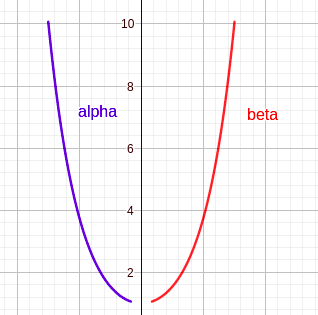
\includegraphics[scale=0.7]{../images/L3_ex3.png}
			\caption{Catetária sob o intervalo (-3,3)}
			\label{ex3}
		\end{figure}
		
		\end{itemize}
		
		
	\item[\ex{4}]\textcolor{blue}{
		Considerando o conceito de derivada como aproximação linear. Considere a aplicação:}
		\blue{
		\begin{align*}
			f(v)&:\rr\to\rr\\
			(x,y)&\to (x^3+y^3,x^3-y^3)
		\end{align*}
	
	determine suas derivadas $f'(v)$ e $f''(v)$
}
	\item[\sol{4}] Pelo jacobiano, considerando $f_1(x,y)=x^3+y^3$ e $f_2(x,y)=x^3-y^3$ a primeira derivada será:
	
	\begin{align*}
		f'(v)&=\displaystyle\begin{bmatrix}
			\dfrac{\partial f_1}{\partial x} & 
			\dfrac{\partial f_1}{\partial y}  \\[3ex] % <-- 1ex more space between rows of matrix
			\dfrac{\partial f_2}{\partial x} & 
			\dfrac{\partial f_2}{\partial y} 
		\end{bmatrix}
	=\begin{bmatrix}
		3x^2 & 
		3y^2  \\[0.5ex] % <-- 1ex more space between rows of matrix
		3x^2 & 
		-3x^2 
	\end{bmatrix}
	\end{align*}
	
	Para a segunda derivada utilizaremos a definição de Hessiana multidimensional para funções vetoriais \cite{wiki:Hessian_matrix}, 
	
	\begin{align*}
		f''(v)&=\bd{H}(f)=(\bd H (f_1),\bd H (f_2)),
	\end{align*}
	
	onde, 
	$
		\bd H (f_1)=\begin{bmatrix}
			\dfrac{\partial^2f_1}{\partial x^2} & 
			\dfrac{\partial ^2f_1}{\partial x\partial y}  \\[3ex] % <-- 1ex more space between rows of matrix
			\dfrac{\partial^2 f_1}{\partial y\partial x} & 
			\dfrac{\partial^2 f_1}{\partial y^2}
		\end{bmatrix} =
	\begin{bmatrix}
		6x & 
		0  \\[0.5ex] % <-- 1ex more space between rows of matrix
		0 & 
		6y
	\end{bmatrix},
	$
	e analogamente $\bd H(f_2)=\begin{bmatrix}
		6x & 
		0  \\[0.5ex] % <-- 1ex more space between rows of matrix
		0 & 
		-6y
	\end{bmatrix}$

Sendo assim, $f''(v)$ é o tensor $\left(\begin{bmatrix}
	6x & 
	0  \\[0.5ex] % <-- 1ex more space between rows of matrix
	0 & 
	6y
\end{bmatrix},\begin{bmatrix}
6x & 
0  \\[0.5ex] % <-- 1ex more space between rows of matrix
0 & 
-6y
\end{bmatrix}\right)$	
	
	\item[\ex{5}] uma aplicação $\Phi:\rr\to\rr$ é dita \textit{movimento rígido} quando preserva distâncias. Isto é:
	
	$$||\Phi(p)-\Phi(q)||=||p-q||$$
	
	Verifica-se que todo movimento rígido se escreve de forma única como composta de uma transformação linear ortogonal e uma translação, ou seja:
	
	$$\Phi(p)=Ap+p_0~\forall p\in\rr,$$
	
	em que, $A:\rr\to\rr$ é um operador linear ortogonal e $p_0$ um ponto de $\rr$. Diz-se que $\Phi$ é \textit{direto} ou \textit{inverso}, conforme $\det(A)=1$ ou $-1$ respectivamente. Verifique que $\Phi$ é diferenciável e calcule $\Phi'(p)$ e $\Phi''(p)$.
	
	\item[\ex{6}] \textcolor{blue}{Mostre que uma matriz de rotação e uma matriz de reflexão são aplicações linearesortogonais e, portanto, podem ser interpretadas como um movimento rígido.}
	
	\item[\sol{6}] Uma matriz $A\in\rn$ é ortogonal se $AA^T=I_n$ onde $I_n$ é a matriz identidade de $n$ dimensões. Considerando o $\rr$, uma matriz de rota~ção é da forma:
	
	$$A=\begin{bmatrix}
		\cos \theta &-\sin\theta\\
		\sin\theta &\cos\theta
	\end{bmatrix},\text{ com }\theta\in\real$$

	Multiplicando pela transposta temos:
	
	\begin{align*}
		&~~~\,\begin{bmatrix}
			\cos \theta &-\sin\theta\\
			\sin\theta &\cos\theta
		\end{bmatrix}\begin{bmatrix}
		\cos \theta &\sin\theta\\
		-\sin\theta &\cos\theta
	\end{bmatrix}\\&=\begin{bmatrix}
	\cos^2 \theta +\sin^2\theta&\cos\theta\sin\theta-\sin\theta\cos\theta\\
	\sin\theta\cos\theta-\cos\theta\sin\theta &\sin^2\theta+\cos^2\theta
\end{bmatrix}\\&=\begin{bmatrix}
1 &0\\
0 &1
\end{bmatrix}
	\end{align*}

	Logo, uma matriz de rotação no plano é ortogonal.
	
	Podemos representar uma reflexão de um ponto por uma reta $L$ que faz ângulo $\theta$ com o eixo das abscissas pela matrix\cite{wiki:Rotations_and_reflections_in_two_dimensions}: 
	
	$$A=\begin{bmatrix}
		\cos(2\theta)&\sin(2\theta)\\
		\sin(2\theta)&-\cos(2\theta)
	\end{bmatrix}$$

	Note que $A=A^T$, se realmente for o caso de $A$ ser orgonal teremos $A^2=I$, que é o esperado de uma reflexão, pois se aplicada duas (ou um número par) vezes devemos voltar ao mesmo lugar. verificando então a ortoginalidade:
	
	\begin{align*}
		&\begin{bmatrix}
			\cos(2\theta)&\sin(2\theta)\\
			\sin(2\theta)&-\cos(2\theta)
		\end{bmatrix}\begin{bmatrix}
		\cos(2\theta)&\sin(2\theta)\\
		\sin(2\theta)&-\cos(2\theta)
	\end{bmatrix}\\
	&=\begin{bmatrix}
		\cos^2 (2\theta) +\sin^2(2\theta)&\cos(2\theta)\sin(2\theta)-\sin(2\theta)\cos(2\theta)\\
		\sin(2\theta)\cos(2\theta)-\cos(2\theta)\sin(2\theta) &\sin^2(2\theta)+\cos^2(2\theta)
	\end{bmatrix}\\&=\begin{bmatrix}
		1 &0\\
		0 &1
	\end{bmatrix}
	\end{align*} 

	\textbf{Q.E.D}


	
	
	
	\end{enumerate}
	
	\newpage
	
	% \addcontentsline{toc}{section}{Referências}
	\bibliographystyle{plain}
	\bibliography{refs}
\end{document}